\section{Container-Orchestrierung}
Compose kann als Single-Host-Container-Orchestrierung betrachtet werden, da es mehrere Container auf einem einzigen Host verwaltet und koordiniert.
Ein Single Host hat den Nachteil, dass es kein Failover gibt, wenn der Host ausfällt, und dass die gesamte Last, die durch die Services verursacht wird, nicht verteilt wird.
Um das zu verhindern, können die Services auf eine Gruppierung von Host-Rechnern, auch Cluster genannt, verteilt werden. Dies ist mit Compose jedoch nicht möglich.
Dafür wird eine Cluster-/Multi-Node-Container-Orchestrierung benötigt. Diese verwaltet die Container über Services, die eine weitere Abstraktionsebene über den Container darstellen.

\subsection{Docker Swarm}
Docker selber bietet als Cluster-Orchestrator Docker Swarm an (zureinfachheit absofort nur Swarm genannt) und ist so mit einer der einfachsten Wege um
vom einen Compose zu einen Cluster-Orchestrator zuwechseln, da weiterhin die compose.yaml verwendet wird.

Die compose.yaml Datei muss dafür mit dem Befehl docker stack deploy ausgeführt werden, dabei setzt Swarm aber vorraus, dass das Gerät zu einen Cluster gehöhrt bzw 
wie es in Swarm heißt, einen Docker-Swarm. Es würd aber nicht verlangt, das der Swarm schon aus mehreren Host besteht,
sondern kann mit dem Befehl docker swarm init, ein Swarm mit nur einen Host auf den Rechner erstellt werden \parencite[vgl. 119]{kofler2023docker}, 
daher kann Swarm auch nur auf einen Node verwendet werden, auch wenn es als Multi-Node ausgelegt ist.

Dennoch besteht ein Swarm immer aus zwei verschiedenen Arten von Nodes. 
Einerseits gibt es die Manager Nodes, die die Cluster-Verwaltung übernehmen, andererseits gibt es die Worker Nodes, auf denen die Container ausgeführt werden. 
Ein Manager Node kann aber auch zusätzlich als Worker Node verwendet werden, beispielsweise wenn der Swarm nur aus einem Node besteht.

Die Vorteile von Swarm im Vergleich zu Compose sind zum einen, dass Swarm direkt auf mehrere Nodes skaliert werden kann und dass die Replikate der Container nun hochskaliert werden können. 
Swarm sorgt mit seiner Cluster-Verwaltung außerdem dafür, dass die Anzahl der Replicas der Container immer gleich bleibt, auch wenn ein Container oder sogar ein ganzer Node ausfällt.
Dieser Zustand wird als Desired-State-Prinzip bezeichnet.

Obwohl Swarm einen einfachen Übergang zu einer Cluster-Orchestrierung bietet, ist es dennoch nicht die optimale Wahl als Cluster-Orchestrator.
Einerseits ist die Anwendung weiterhin an Docker-Techniken gebunden, andererseits ist Swarm nicht so stark verbreitet, weswegen es eine kleinere Community hat.
Dadurch ist Swarm weniger erweiterbar und flexibler als andere Cluster-Orchestratoren.

\subsection{Kubernetes}

Kubernetes bietet mit einer größeren Community, vielen guten Erweiterungen und ausführlichen Domkumentationen
zum vergleich zu Swarm, trotz höhrer Komplexität, gute Vorteile \parencite[vgl. 452]{kofler2023docker}.
Dabei darf Kubernetes nicht als Erweiterung von Docker angesehen werden, sondern als eigenständiges System.
Kubernetes verwendet eine Container Runtime Interface (CRI), weshalb weitere Runtimes verwendet werden können. Dadurch ist Kubernetes nicht auf Docker beschränkt.

Daher wird sich dieser Teil zuerst mit der Architektur beschäftigen und anschließend die Objekte und Ressourcen von Kubernetes vorstellen.

\subsubsection{Architektur}

Wie bei Swarm besteht Kubernetes aus zwei verschiedenen Arten von Knoten: den Master-Knoten und den Worker-Knoten.
Die Master Nodes werden auch Control Plane genannt und die Worker Nodes.
Ebenso wie in Swarm übernimmt der Master Node die Verwaltung des Clusters, während auf dem Worker Node die Container Engine läuft.

\begin{figure}[htbp]
\centering
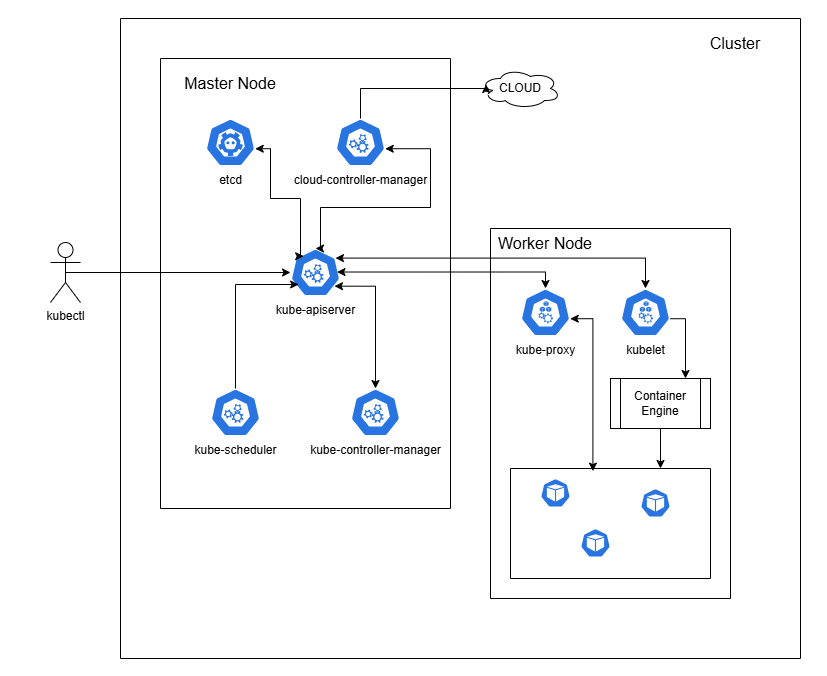
\includegraphics[width=0.8\textwidth]{bilder/grundlagen/kubernetes-architektur.png}
\caption{Kubernetes-Architektur}
\label{fig:kubernetes_architektur}
\end{figure}

Ein Master Node verfügt über einen kube-apiserver, der sowohl für die Kommunikation zwischen den Nodes als auch für die externe Kommunikation zuständig ist.
Über diesen steuert der Master Node den Cluster, d. h. er entscheidet auch darüber, ob neue Ressourcen angelegt oder überarbeitet werden. Der kube-apiserver kontrolliert, ob die Ressourcen, Limits und Quotas eingehalten werden.
Der kube-apiserver stellt auch die einzige Verbindung zur etcd-Datenbank im Master Node her. In der etcd-Datenbank stehen die Manifeste der Ressourcen des Clusters, daher ist dort auch der aktuelle Zustand des Clusters zu finden.
Auf dem Master Node befinden sich auch der Kube-Scheduler und der Kube-Controller-Manager, die für die Verwaltung des Clusters zuständig sind. Der Kubelet-Scheduler weiß, wie viel Ressourcen auf den Nodes und ihren Containern verbraucht werden und wie viel übrig sind.
Darüber hinaus steuert er das Pod-Scheduling, also die Verteilung der Pods auf den Nodes. Der kube-controller-manager übernimmt die Überwachung der laufenden Prozesse und reagiert auf Ereignisse. Beispielsweise verteilt er die Pods eines Nodes, der ausgefallen ist, auf die anderen Nodes.
Beide sind wiederum über den kube-apiserver erreichbar. Zu guter Letzt ist im Master Node auch der cloud-controller-manager enthalten, der die Kommunikation zu den Cloud-Diensten übernimmt und auch über die Cloud gesteuert werden kann, wenn der Cluster in einer Cloud betrieben wird.

Ein Cluster besteht auch üblich aus mehreren Worker Nodes. Diese übernehmen keine Verwaltung des Clusters sondern nur die Ausführung der Container. Dadurch sind die Worker Nodes austauschbar und  können auch ausfallen \parencite[vgl. 51]{welter2024kubernetes}. 
Auf dem Worker Node läuft die Controller Engine, die die Container betreibt.
In Kubernetes laufen die Container jedoch nicht direkt auf den Nodes, sondern in Pods, die auf den Nodes ausgeführt werden. Auf einem Node können mehrere Pods laufen.
Ein Worker Node besitzt ein Kubelet und einen Kube-Proxy. Letzteres verwaltet die Kommunikation zwischen den Pods und dem restlichen Netzwerk des Clusters. 
Das Kubelet verwaltet die Pods auf dem Worker Node. Es führt die Pods über die Controller Engine aus und überwacht diese.
Kubelet und Kube-Proxy sind direkt mit dem Kube-Apiserver von mindestens einem Master-Node verbunden. Der Kube-Apiserver beauftragt beispielsweise den Kubelet, einen Pod zu deployen. Dafür schickt er das Manifest des Pods an den Kubelet.
Ein Master Node hat ebenfalls ein Kubelet und einen Kube-Proxy, da zur Verwaltung des Clusters auch Pods auf ihm laufen. Der Master Node sollte jedoch nicht als zusätzlicher Worker Node genutzt werden.
\FloatBarrier
\subsubsection{Manifeste}

Die Objekte von Kubernetes, wie beispielsweise Pods, Deployments und ConfigMaps, werden mithilfe von Manifesten festgelegt. 
Diese Manifeste sind normalerweise YAML-Dateien, die den Aufbau, das Verhalten, die Befugnisse und auch den Inhalt der Objekte beschreiben. 
Kubernetes selber sagt das für Manifeste auch JSON genommen werden kann \parencite{kubernetesObjects}, dies ist jedoch eher unüblich.
Manifeste unterscheiden sich je nach Objekt, dennoch gibt es grundlegende Informationen, die angegeben werden müssen.
Dazu gehört, welches Objekt mit Kind erstellt werden soll und welche Version des Objekts mit Apiversion genutzt werden soll. 
Zusätzlich müssen grundlegende Informationen über das Objekt unter Metadaten beschrieben werden, wobei mindestens der Name des Objekts angegeben werden muss. 
Danach kann unter „spec” der gewünschte Zustand und das Verhalten des Objekts festgelegt werden.

\begin{lstlisting}[language=yaml, caption={Beispiel von einen Manifest}]
apiVersion: v1
kind: Pod
metadata:
    name: my-pod
spec:
    ...
\end{lstlisting}
\subsubsection{Pods}

Wie schon erwähnt wurde laufen auf einen Node mehrere Pods. Im Pod wiederrum werden einer oder mehrere Container ausgeführt und gemanged.
Um die Container auszuführen benutzt Kubernetes das Container Runtime Interface (kurz CRI) benutzt, damit noch andere Runtimes als nur die von Docker genutzt werden können \parencite[vgl. 108]{welter2024kubernetes}.
Anders als bei Compose erstellt Kubernetes die Images nicht mehr selbst, sondern holt sie sich aus Container-Registern.

Wie viele Container in einen Pod laufen sollen, kann selbst entschieden werden, es gibt jedoch Möglichkeiten, wie dies am besten entschieden werden kann.
Wenn man sich an der Separation of Concerns orientiert, dann sollte von keiner der Container der eigenen Anwendung in den gleichen Pod laufen, es sei denn, die Container müssen gemeinsame Ressourcen teilen oder die Container dürfen nicht auf unterschiedlichen Nodes laufen.
Es können aber auch kleinere Container in einen Pod hinzugefügt werden, die die Hauptanwendung verbessern, z. B. durch zusätzliches Logging oder einen Proxy. Dabei ist es aber wichtig, dass diese entkoppelt sind von der Hauptanwendung. Falls dies nicht zutrifft, z. B. weil es die Skalierung beeinflusst, wäre es besser, diese zu trennen.
Diese Art von Container wird auch Sidecar-Container genannt.

\subsubsection{Deployments}

Von einem Pod kann es beliebig viele Duplikate geben. Dies wird jedoch nicht im Pod selbst festgelegt, sondern im ReplicaSet.
Ein ReplicaSet erstellt die Pods und sorgt dafür, dass die Anzahl der Replikate der Pods gleich bleibt.
Dabei wird im ReplicaSet festgelegt, wie viele Pods ein Service haben soll.
Fällt ein Pod aus, erstellt das ReplicaSet einen neuen. Über das ReplicaSet kann auch die Anzahl der Pods skaliert werden.

Kubernetes selber empfield, aber nicht ReplicaSets selber zu nutzen, sondern in einen Deployment \parencite{kubernetesReplicaSet}.
Ein Deployment kann selbst ein ReplicaSet erstellen und dieses verwalten. Ein Deployment verwaltet daher über sein ReplicaSet dessen Pods.
\begin{figure}[htbp]
\centering
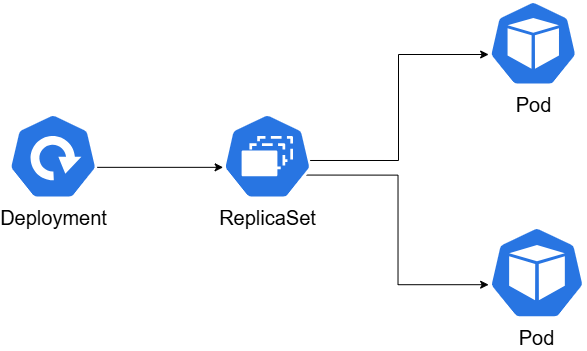
\includegraphics[width=0.8\textwidth]{bilder/grundlagen/deploymentflow.png}
\caption{Deployment-Architektur}
\label{fig:deploymentflow}
\end{figure}
\FloatBarrier

\subsubsection{Service}

Kubernetes baut ein eigenes internes Netzwerk auf, über das die Pods miteinander kommunizieren können und erreichbar sind.
Dabei erhält jeder Pod eine eigene IP-Adresse, allerdings ist ein Pod kurzlebig. Wenn ein Pod ausfällt und ersetzt wird, hat der neue Pod nicht die gleiche IP-Adresse wie der Pod davor.

Damit die Pods mit einer festen IP-Adresse erreicht werden können, gibt es in Kubernetes Services, die alle Replicas eines Pods kennen.
Zusätzlich dient ein Service als Loadbalancer, der den Datenverkehr auf die Pods verteilt.
Die Kommunikation findet daher nicht über die Pods selbst, sondern über deren Service statt.
\subsubsection{Ingress}

Ein Kubernetes-Cluster kann, wenn er Daten von außen benötigt, diese einfach abrufen. Wenn jedoch eine Anwendung im Cluster außerhalb des Clusters erreichbar sein soll, muss dies zuerst eingerichtet werden.

Wenn nur eine TCP-Verbindung benötigt wird, kann ein Service vom Typ NodePort erhalten werden. Wenn jedoch eine HTTP-Verbindung benötigt wird, wird ein Ingress benötigt.

Ein Ingress erhält dabei die Anfrage von außen und leitet sie an den passenden Service weiter. Dies kann über den Host oder den Pfad einer URL entschieden werden.
Über den Ingress können auch TLS-Zertifikate eingefügt werden, um HTTPS-Verbindungen zu erstellen.
\begin{figure}[htbp]
\centering
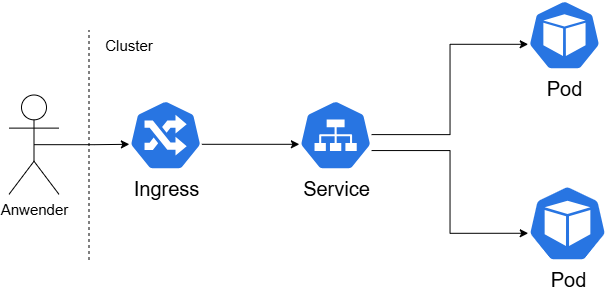
\includegraphics[width=0.8\textwidth]{bilder/grundlagen/kommunikation.png}
\caption{Kommunikation mit Ingress und Service}
\label{fig:kommunikation}
\end{figure}
\FloatBarrier
\subsection{Zuverlässigkeit durch Kubernetes}

Kubernetes bietet durch seine Technik einige Features, die genutzt werden können, um die Zuverlässigkeit zu erhöhen.

Dies beginnt damit, dass Kubernetes mehrere Replikate von Pods hat, wodurch sich die Verfügbarkeit verbessert. Selbst wenn ein Pod eines Services ausfällt, z. B. eines Backends, ist dieser dennoch verfügbar, da der Traffic auf die Replikate umgeleitet wird.
Dies kann durch die Eigenschaft von Kubernetes als Cluster-Container-Orchestrator gesteigert werden, da die Anwendungen auf mehreren Nodes laufen. Deshalb bleibt die Anwendung auch bei einem Node-Ausfall bestehen, während bei einem Single-Host-Container-Orchestrator die gesamte Anwendung down wäre.
Dies kann bei Kubernetes auch verknüpft werden, indem im Deployment eingestellt wird, dass sich die Replicas von Pods desselben Services auf verschiedene Nodes verteilen. Dadurch bleibt der Service auch bei einem Node-Ausfall erreichbar.
Dabei punktet Kubernetes auch beim Aspekt der Fehlertoleranz, da es erkennt, wenn ein Pod ausfällt – egal aus welchem Grund – und den Traffic auf die noch existierenden Replicas dieses Pods umleitet.

Kubernetes verfolgt das Desired-State-Prinzip, weshalb es bei einem Pod-Ausfall direkt versucht, den Pod wiederherzustellen, damit die Anzahl der Replicas dieses Pods gleich bleibt, wie es im Deployment angegeben ist.
Bei einem Ausfall eines ganzen Nodes versucht Kubernetes, die Pods auf einem anderen Node wiederherzustellen. Sobald ein neuer Node im System hinzugefügt wird oder der alte Node wiederhergestellt wurde, kann Kubernetes diese Pods erneut verteilen.

All dies gehört auch zum Self-Healing von Kubernetes und kann die Zuverlässigkeit von Anwendungen weiter verbessern.
Kubernetes überwacht die Gesundheit der Pods durch Probes. Dadurch kann erkannt werden, ob der Container im Pod noch richtig läuft. Falls nicht, würde Kubernetes den Pod als ungesund markieren und den Traffic auf die anderen Pods dieses Services umleiten.
Zusätzlich versucht Kubernetes, den Container im Pod oder sogar den ganzen Pod neu zu starten.  Dadurch können Fehler im System vermieden und der richtige Betrieb wiederhergestellt werden.

Das Desired-State-Prinzip muss in Kubernetes aber nicht fest sein, sondern kann auch automatisch nach Last skaliert werden, und zwar durch den Horizontal Pod Autoscaler. 
Dieser kann die Anzahl der Replicas eines Pods erhöhen und auf eine angegebene maximale und minimale Anzahl beschränken, je nachdem, wie viel Last ein Service verbraucht.
Dies verstärkt die Stabilität im System, da die Ressourcen angemessen verteilt werden.

Kubernetes erhöht auch die Zuverlässigkeit durch Rolling Updates. Bei einem Rolling Update wird ein Pod nach dem anderen ausgetauscht, während das Update läuft. Dadurch können Ausfälle während einer Aktualisierung vermieden werden.
Dies kann durch die Probes, die im Self-Healing verwendet werden, verbessert werden, indem zuerst geprüft wird, ob der Pod gesund ist, bevor er für den Traffic freigegeben wird.
